\documentclass[hidelinks,12pt]{article}
\linespread{1.3}
\usepackage{hyperref}
\usepackage{enumerate,changepage,lipsum,titlesec, longtable}
\usepackage{cite}
\usepackage{comment, xcolor}
\usepackage[pdftex]{graphicx}
  \graphicspath{{images/}, {images/stat/}}
  \DeclareGraphicsExtensions{.pdf,.jpeg,.png, .jpg}
\usepackage[cmex10]{amsmath}
\usepackage{tikz}
\usepackage{array} 
\usepackage{subfigure} 
\newcommand{\grey}[1]{\textcolor{black!30}{#1}}
\newcommand{\red}[1]{\textcolor{red!50}{#1}}
\newcommand{\fref}[1]{Figure \ref{#1}}
\newcommand{\tref}[1]{Table \ref{#1}}

% tikz package specs
\usetikzlibrary{calc,trees,positioning,arrows,chains,shapes.geometric,%
    decorations.pathreplacing,decorations.pathmorphing,shapes,%
    matrix,shapes.symbols}

\tikzset{
>=stealth',
  punktchain/.style={
    rectangle, 
    rounded corners, 
    % fill=black!10,
    draw=black, very thick,
    text width=30em, 
    minimum height=3em, 
    text centered, 
    on chain},
  line/.style={draw, thick, <-},
  element/.style={
    tape,
    top color=white,
    bottom color=blue!50!black!60!,
    minimum width=8em,
    draw=blue!40!black!90, very thick,
    text width=10em, 
    minimum height=3.5em, 
    text centered, 
    on chain},
  every join/.style={->, thick,shorten >=1pt},
  decoration={brace},
  tuborg/.style={decorate},
  tubnode/.style={midway, right=2pt},
}

\oddsidemargin0cm
\topmargin-2cm %I recommend adding these three lines to increase the
\textwidth16.5cm %amount of usable space on the page (and save trees)
\textheight23.5cm

\makeatletter
\renewcommand\paragraph{\@startsection{paragraph}{4}{\z@}%
            {-2.5ex\@plus -1ex \@minus -.25ex}%
            {1.25ex \@plus .25ex}%
            {\normalfont\normalsize\bfseries}}
\makeatother
\setcounter{secnumdepth}{4} % how many sectioning levels to assign numbers to
\setcounter{tocdepth}{4}    % how many sectioning levels to show in ToC


\begin{document}
\title{Developing District System Design Support Package \\
       \large Computer Tool Survey and Function Specification}
\maketitle
\tableofcontents
\newpage
\section{General Introduction}
IDEA created a guide document to help planners and developers to
create energy maps. \fref{fig:energyMapIDEA} shows the contents that
could be included in energy maps: sustainable energy source (water
body, biomass, wind, hydropower) location and district heating
locations. The creation of energy maps happens after setting up the
community district energy project objectives. It involves data
collection of ``building density, mix of uses, and anchor loads''\cite
{IDEA2012} and data assembling and map creation.

Definition of energy map: ``a map showing opportunities and
constraints for clean and renewable energy projects across a given
area. This will incorporate thermal demand data typically presented in
a heat map''~\cite{IDEA2012}.  

Definition of heat map: ``map showing locations where heat demand is
sufficient to support district heating. Often included as part of an
energy map.''~\cite{IDEA2012}
\begin{figure}[h!]
  \centering
  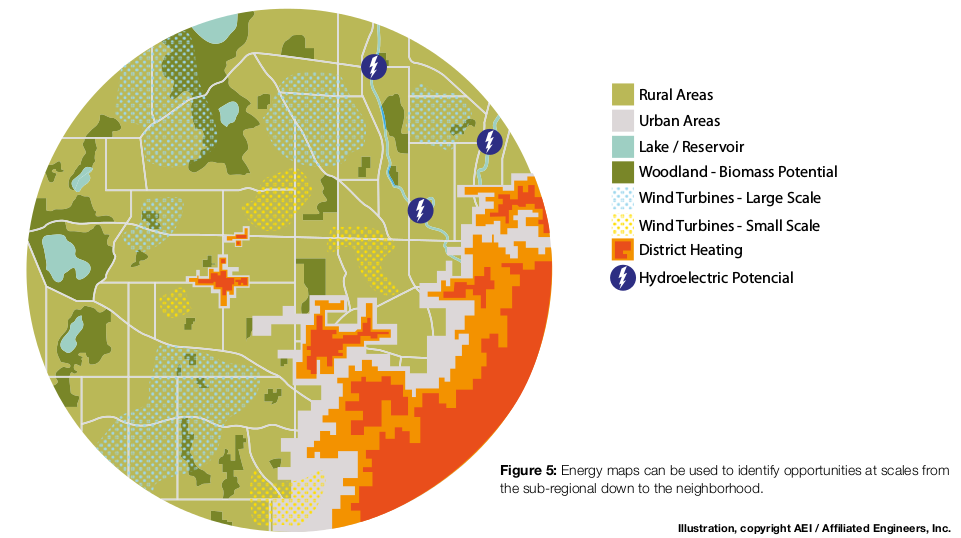
\includegraphics[width=0.7\linewidth]{energyMapIDEA.png}
  \caption{IDEA schematic energy map~\cite{IDEA2012}}
  \label{fig:energyMapIDEA}
\end{figure}

The work flow of the energy map creation and the information involved
in the process are as follows (adapted from \cite{IDEA2012})
\begin{enumerate}[{Step }1]
\item \textbf{Objective Setting}
  \begin{itemize}
  \item People;
  \item Planet;
  \item Profit;
  \end{itemize}
\item \textbf{Data collection}
  \begin{itemize}
  \item Land use density
  \item Energy Demand (hourly scale~\cite{Baird2014})
    \begin{itemize}
    \item Current energy consumption for existing buildings
    \item Future energy consumption for potential new development
      \begin{itemize}
        \item new development rate
        \item improvement of building energy efficiency,
        \item improvement of people's energy use behavior
        \end{itemize}
      \end{itemize}
    \item Building age (used to calibrate building energy consumption
      prediction or assessment)
    \item Current and future anchor load buildings
    \item Energy sources
      \begin{itemize}
      \item Renewable: solar, wind, geothermal, biomass, water body
      \end{itemize}
    \item Energy delivery system;
      \begin{itemize}
      \item Existing district network
      \end{itemize}
    \end{itemize}
  \item \textbf{Analysis}\label{step:analysis}
    \begin{itemize}
    \item classify urban area according to their different energy
      solutions (``energy character area''\cite{IDEA2012}): in
      \cite{IDEA2012}, an example of defining the ``energy character
      area'' is as follows: for residential suburban area, which has
      low density and low degree of mixed land use, a suitable energy
      strategy is small scale energy generation system, such as solar
      energy); for center city area, with high density, a large
      district energy system with CHP is suitable.
    \item ``suitability of low carbon technology''~\cite{IDEA2012}
      \begin{itemize}
      \item Basic function
        \begin{itemize}
        \item Development scale
        \item Service area
        \item Energy supply profile
        \item ``Implications for phasing''~\cite{IDEA2012}
        \item Constraints: land use, zoning regulation etc.
        \end{itemize}
      \item People
      \item Planet
        \begin{itemize}
        \item Annual total $CO_2$ emission
        \item ``Ability to integrate local or renewable fuel
          sources.''~\cite{IDEA2012}
        \end{itemize}
      \item Profit
        \begin{itemize}
        \item cost, 
        \item profit,
        \item payback period.
        \end{itemize}
      \end{itemize}
    \item site analysis based on data from the previous step and land
      use constraint
    \end{itemize}
\end{enumerate}

From this analysis above, the current dynamic energy map has
information of ``Current energy consumption'' but lacks the other
information.

IDEA document described the role of energy maps ``help identify
opportunities for new energy project, determine suitable technologies
and approaches to energy generation, distribution and supply,
highlight opportunities to link to other projects or share energy
centers; and aid decisions about prioritizing
projects''~\cite{IDEA2012}. Energy mapping is especially helpful in
step \ref{step:analysis} Analysis.

According to IDEA document, energy maps can show:
\begin{itemize}
\item what sites are available (free of constraints)
\item what energy strategy is possible for a site.
\item what sites are with good energy potential that supports new
  development
\item what project should be developed first.
\end{itemize}

Energy maps can influence energy strategy by: ``encouragement of
renewable energy generation in appropriate areas by green permitting,
retrofit weatherization programs in areas of older buildings,
ordinance requiring disclosure by commercial building owners of energy
efficiency standards, setting code standards for new construction, and
specifying district energy systems for appropriate
areas.''~\cite{IDEA2012}
\newpage
\bibliographystyle{plain}
\bibliography{myCitation}
\end{document}